\chapter{Analysis}\label{analysis}

\section{Known approaches}\label{known-approaches}

The idea of distributed computing has been known since the 70's.
Different approaches have been tried since then. Some of them are
described in this section in order to show different concepts.

\subsection{Client/server architecture}\label{clientserver-architecture}

It's very common example of centralized system. In this pattern is one
central node, known as the server. The rest of nodes, clients, are all
connected to it. All the information is stored at the server. Also all
the important computations happen there. The communication is typically
initialized by the client, which sends a request. The server processes
it and returns the desired result. Pros of this approach are relatively
simple implementation and easy control of the traffic, because all the
data passes through server. Also the data flow can be controlled easily.
However the huge disadvantage is, that the server is by definition a
single point of failure, i.e.~if it goes down, the whole system becomes
unusable. Also, thanks to the asymmetric nature of the system, there
usually has to be more parts of the software, one to run on the server
and the other to run on the clients. The system is dependent on the
server's performance too.

\subsection{Peer to peer
architectures}\label{peer-to-peer-architectures}

\citep{SupPeer} \subsection*{Pure peer to peer network} Peer to peer
paradigm is virtually the opposite of the previous model. Nodes are
completely equivalent to each other. Any of them can join the network at
any time, as well as leave it. This approach means great scalability and
fault tolerance. On the other hand, it requires more complex design and
can encounter problems with security and management of the network. Our
framework implements this model.

\subsection*{Hybrid peer to peer network}

This approach combines the previous two. There exists one node which is
dedicated to serve as a control server. Each node contacts this server
and all the control information pass through it while the data are
exchanged in the same manner as in the pure peer to peer networks. This
approach removes possible problems with the control of the data flow and
provides information coherence while scalability is preserved. However,
the issue with the single point of failure is reintroduced here.

\subsection*{Super peer architecture}

Another try to improve the architecture introduces the concept of the
so-called super peer. It is a computer, usually with slightly better
performance than other nodes, that plays the role of the control server,
but only for a restricted group of nodes. Autonomous groups (clusters)
are thus formed. It has the same advantages as the hybrid network but
the potential super peer failure is not so crucial. Also each super peer
can have backup so the robustness of the network can be very good.

\subsection{Summary}\label{summary}

We showed different implementations of the idea of distributing the
work. Each has its own specifics and may be suitable for some
application. We have chosen to implement our framework to conform to the
pure peer to peer paradigm as much as possible. Although the super peer
architecture offers better control, we decided not to use it for several
reasons. Mainly because our framework is supposed to be used in rather
small networks where this paradigm could be quite exaggerated. Also we
did not use the hybrid network because we definitely want to avoid
presence of the single point of failure.

\section{Existing solutions}\label{existing-solutions}

Since encoding of the video files is quite reasonable task, there was a
few implementations of the similar issue. Some of them served for
academic purposes only, but others found good use case in practice.

\subsection{DVE (Distributed Video
Encoding)}\label{dve-distributed-video-encoding}

D. Hughes and J. Walkerdine from the Lancaster university published in
their paper a solution which is using Lancaster's P2P Application
Framework. They implemented a Java plug-in for this framework which uses
Microsoft Windows Media Encoder
SDK\footnote{https://en.wikipedia.org/wiki/Windows\_Media\_Encoder}.
Their approach was quite similar to ours and they achieved quite
persuasive results. However their solution was usable in the specific
environment only.\citep{DVE}

\subsection{Apache Hadoop}\label{apache-hadoop}

It is sophisticated distributed framework written for the Java platform.
It serves for processing large amount of data and also as a storage. It
provides very good ability to deal with hardware failures. The framework
consists of the HDFS (Hadoop Distributed File System) and the processing
part. The HDFS is a distributed file system which uses
TCP/IP\footnote{https://en.wikipedia.org/wiki/Internet\_protocol\_suite}
sockets for communication between nodes. It uses replication of data to
achieve reliability. It is optimized to store large immutable files
(range of gigabytes or even terabytes). The framework could use
different file system, however, one of its main advantages is the
knowledge about the data locality, hence unnecessary data transfers can
be avoided. This feature may not be available when using some different
file system. The processing part is based on the MapReduce engine, based
on functional programming concept. It basically consists of three steps.

\begin{enumerate}
\item Map - A special function is applied to the local data on each worker node, data are associated with a key. This step can be processed in parallel.
\item Shuffle - The data are redistributed, according to keys. Each worker node obtains data sets with the same key
\item Reduce - The data are processed, in parallel.
\end{enumerate}

A special master node is needed which ensures effective task scheduling.
Generally, the framework is suitable for processing large data sets. It
needs dedicated infrastructure and can achieve very good results. It can
be used in many different applications including image processing,
marketing analysis or data mining. It differs a lot from our solution -
among its complexity and suitability for wide range of tasks, it needs
some nodes with special functionality and also the network of
specialized nodes. In contrast, our solution can operate in almost any
computer network and the computing nodes can serve for other
purposes.\citep{Hadoop} \citep{MapRed}

\subsection{BOINC (Berkeley Open Infrastructure for Network
Computing)}\label{boinc-berkeley-open-infrastructure-for-network-computing}

It is a distributed system, developed on the Berkeley university, which
utilizes computing power of personal computers around the world and
interconnects them in the huge network. It supports multiple operating
systems (the client part). Anyone can voluntarily join the network and
scale it up by granting his computer's performance. After installing the
client application, the system is able to exploit free CPU or GPU
capacity of the computer. The server provides him with a portion of the
given task. After the computation, the results are verified and
uploaded. The system is used mainly for scientific computations. For
example it is used by the well known project SETI@home. The framework is
based on the client-server architecture. The server runs on UNIX
OS\footnote{https://en.wikipedia.org/wiki/Unix}, using common
technologies such as the Apache web server and the MySQL database
server. A PHP language is used.There are also CGI programs and daemons
running on the server. The obvious difference is in use of the
client-server model, nevertheless the philosophy of using regular
computers as the computing nodes corresponds to ours. \cite{BOINC}

\subsection{Gnutella}\label{gnutella}

Gnutella is a peer to peer framework used for file sharing. The nodes
use flood technique with limited number of hops for searching of the
desired data. The positive acknowledgement message is sent when this
data was found, employing the UDP protocol. The file transfer can be
negotiated then. The system is based on the super peer architecture,
which makes it possible to reduce maximum number of hops. Though it is
not used for distributed computation, the data transfers are used which
makes it comparable with our system.\citep{Gnutella}

\subsection{BitTorrent protocol}\label{bittorrent-protocol}

Another interesting file sharing technique is introduced in the
BitTorrent network. The files offered by the node are stored in special
list and a single file download can (and usually do) use more nodes.
This is possible, because the files are divided into pieces and when the
node downloads some piece, it becomes source of this piece for the
others. The pieces are marked so they can be downloaded in random order.
The system provides good redundancy. Another advantage is, that as the
file spreads through the network, the requirements on original
distributor's bandwidth decrease. Eventually the node could not be
needed at all. This protocol is used for file sharing by the BOINC
framework, among many others. It is certainly an interesting alternative
to handle the file transfers. In our framework, the use of this protocol
would not be very convenient and useful, since once the chunk is
processed, it becomes useless.\citep{BitTor}

\section{Framework description}\label{framework-description}

\subsection{Basic overview}\label{basic-overview}

The heart of the program is one executable file, that should be
accompanied by the configuration file. This is discussed in detail in
\hyperref[installation-and-use]{appendix A}. Main options that should be
set are IP address and a number of port which the program should listen
on. It is also essential to provide credentials (i.e.~address and port)
of some node which should be contacted by default. When more nodes are
spawned, the network is formed and the computation may be initialized.
Note that the information about neighbors spread in a nondeterministic
manner, it matters who is contacted by whom. So it's good to have one or
more nodes which are online most of the time and the rest contacts only
these nodes initially. Otherwise the distribution of the neighborhood
knowledge may be quite slow. Once the network is established, the
computation can begin. If one (or more) nodes have tasks to be done, it
can start the process. The file is then processed and divided into
chunks in the initiating node. These chunks are distributed among
neighbors, processed and returned back. Once the initiator has all
chunks back, it joins them together and the process ends.

C++ language has been chosen for the implementation. It allows us to use
standard POSIX socket
\footnote{https://en.wikipedia.org/wiki/Berkeley\_sockets} API
(Application Programming Interface) which is widely used and has been
proven by thousands of applications. Also it provides convenient
functionality thanks to its Standard Template Library while allowing to
use C library functions so it can cooperate well with the OS. Because it
compiles to the native code, it does not need any interpreter, so its
requirements are lower than other languages' such as Java and C\#. This
fact is positive, because it means, that if the application runs in
background and computes nothing, it does not spend many system
resources. The program is supporting Linux operating system, it has been
tested on several Linux distributions. Nevertheless, it conforms to the
POSIX standard
\footnote{https://en.wikipedia.org/wiki/POSIX\#POSIX.1-2001}, so after
some modifications it could be used with any UNIX or UNIX-like operating
system.

\subsection{Neighbor maintaining}\label{neighbor-maintaining}

The diagram which describes the process can be seen in the Figure 1.1.
When the node wants to use other computer's computation capacity, it
naturally has to contact them first. But the node has no prior explicit
knowledge of the network's infrastructure, moreover, this infrastructure
can change dynamically. To solve this, each node maintains the list of
its neighbors. It contains addresses of the nodes which it has contacted
successfully in the past. The list is refreshed periodically, so the
node keeps track of the current network state. Besides this main list
exists another list, which contains potential neighbors. Generally, each
node that has communicated with the given one sometime in the past is
added to the list of potential neighbors. The purpose of this list is to
reduce the amount of time spent with maintaining the neighbors list.
That is, no more than required count of neighbors is maintained, but if
needed, suggestions can be found in this backup list.

Neighbors are uniquely identified by the pair consisting of address and
communicating port. This is sufficient for the potential neighbors,
because before the neighbor is added to the main list, it has to be
contacted. Additional information is then added, so more complex
structure is needed for storing neighbors. This structure contains
information about neighbor's quality, last known state etc. The quality
of the neighbor helps to prefer one neighbor to another while picking
the one to contact. It is updated after each chunk is delivered from the
given neighbor and reflects the neighbors computation power together
with the speed of the connection.

\subsection*{Initialization and discovery}

This may be the most important part of the process. Its overview is
given in Figure 1.1. The node is provided with the address and port of
the neighbor which should be contacted by default, that is, when the
neighbors list is empty. Each node has minimum count of neighbors which
should be in its list. This number is checked periodically. In case that
the count of confirmed neighbors is too small, the list of potential
neighbors is checked. If it's empty, the node has to obtain more
neighbors so it picks one of its neighbors, contacts it and receives
some suggestions. If it has no neighbors, the default node is contacted.
Once the suggestions are received, the node adds the new addresses to
the list of potential neighbors. When the list contains some potential
neighbors, the node can contact them, confirm, and add as regular
neighbors.

\begin{figure}[h]
\begin{center}
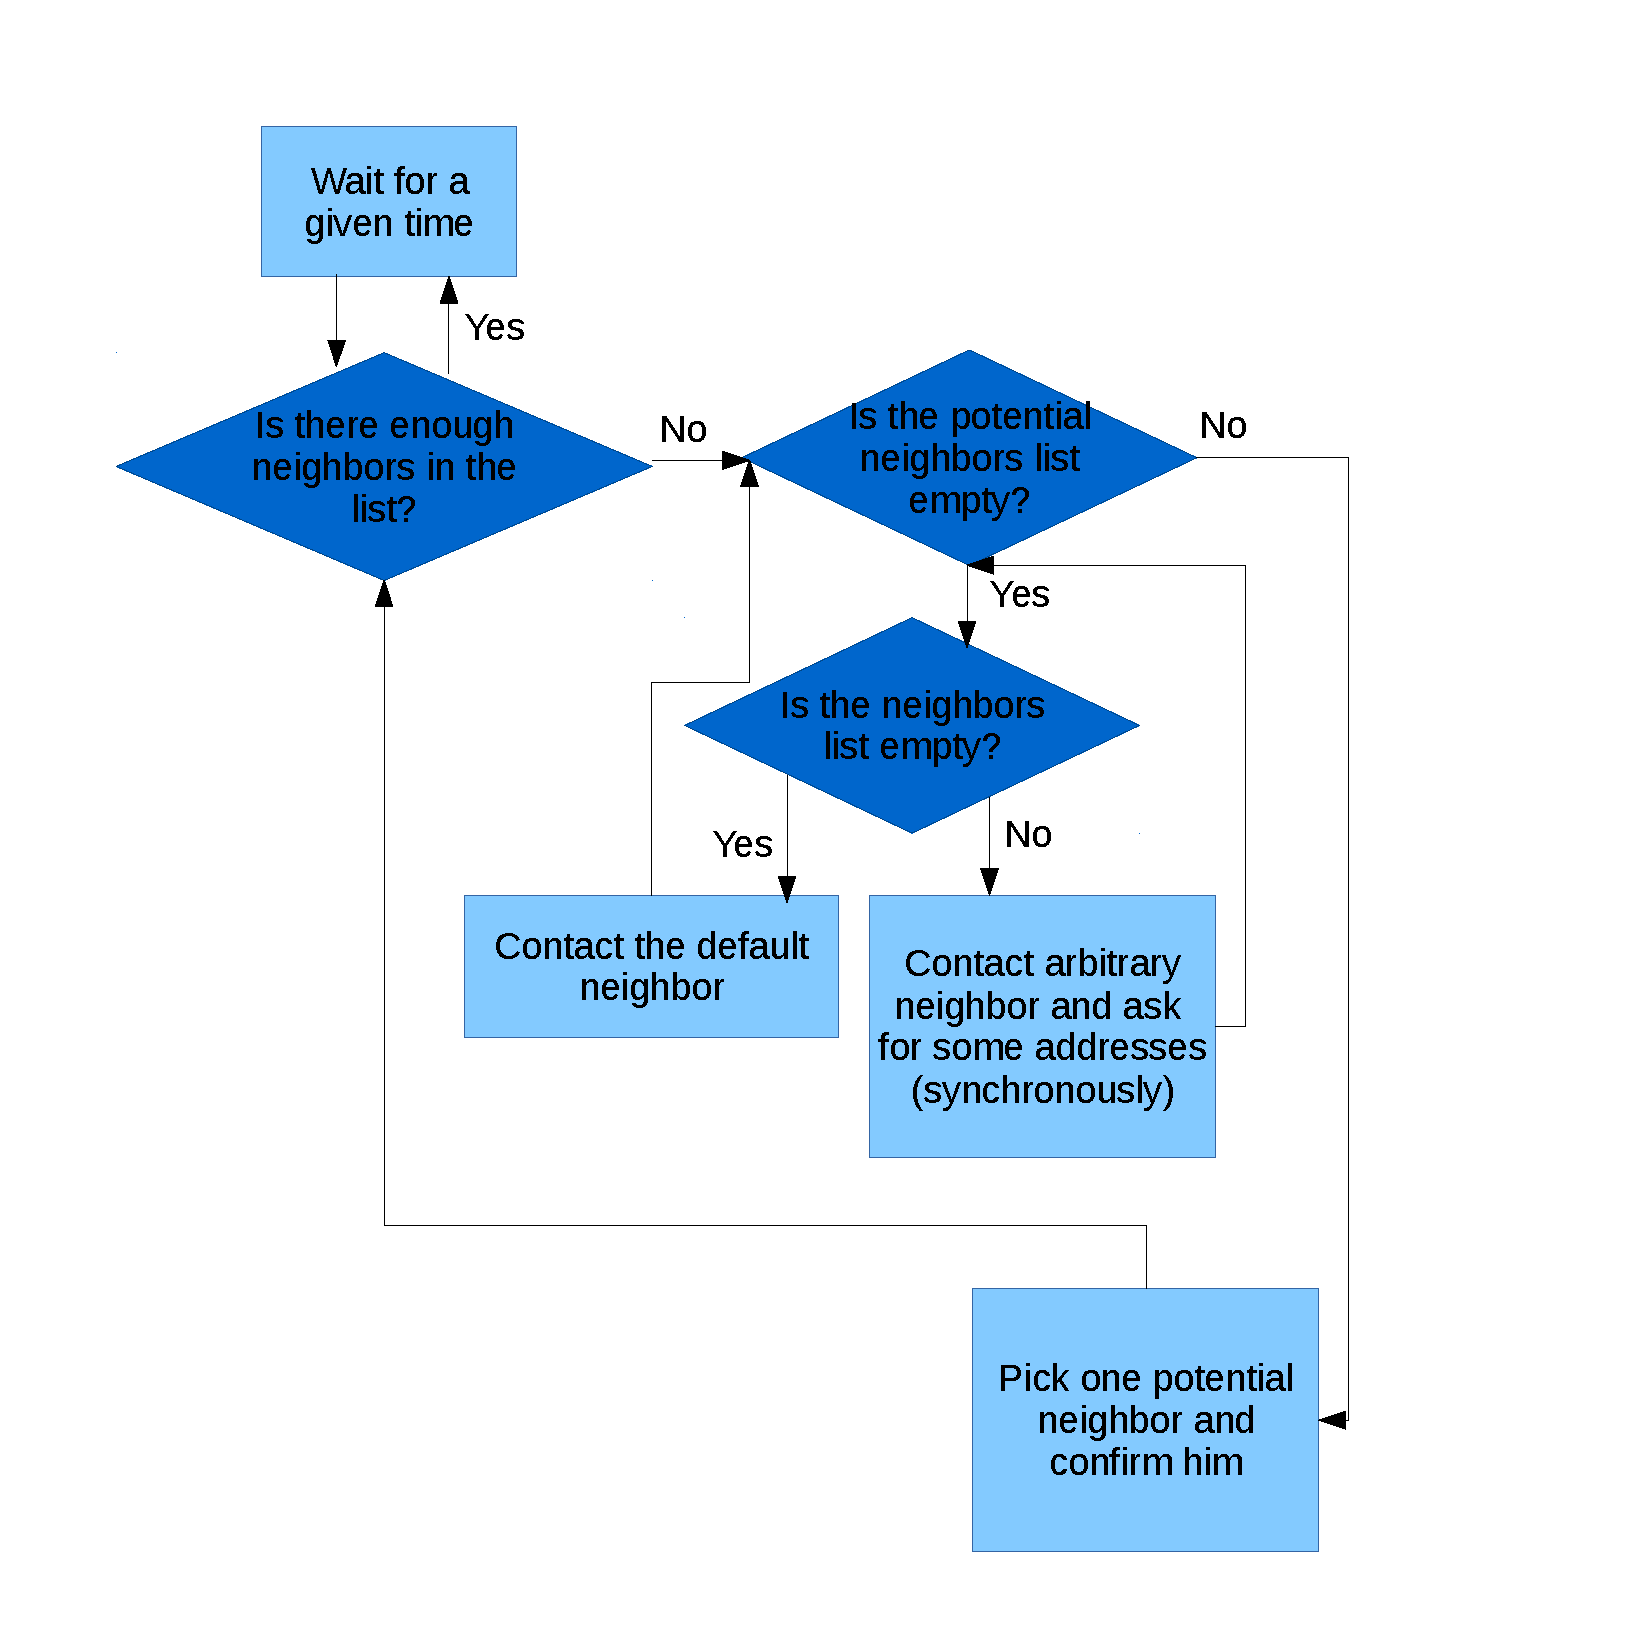
\includegraphics[scale=0.40]{./img/workflow_neighbors.pdf}
\caption{Maintaining the neighbors}
\end{center}
\end{figure}

\subsection*{Gathering neighbors}

When the initiating node has not enough neighbors and it needs more
neighbors with free computation power, it can use another mechanism to
collect them. This mechanism uses a flood technique to spread the
request among the nodes in the network. The request is send to each
neighbor, which spreads it further in the same manner. However, the
request is equipped with time to live value that is decreased after each
hop. Because of this, it does not spread forever nor too far. Once the
node receives a request and is not busy, it contacts the initiator
directly. It can then add him to the list of potential neighbors and
later possibly as the regular neighbor.

\subsection*{Withdrawing from the network}

When the node wants to leave the network it has to abort the process, if
it is the initiator. Then a special message is sent to each neighbor,
which informs them so they can react accordingly. That is, if the
neighbor has tasks to be processed for the leaving one, it removes them
from the queue and then removes the neighbor itself. Removed neighbors
are completely lost, they are no longer stored in either of the lists.
The process of saying goodbye to neighbors is asynchronous, the
withdrawing node does not wait for any confirmation. There are several
reasons for this behavior. Waiting for the response could cause a
deadlock under some specific circumstances, e.g.~if the contacted
neighbor went down unexpectedly. Also, there is no need for it, since
there is no possibility to stop the node from withdrawing.

\subsection*{Neighbor's failure}

There is no guarantee that all the neighbors leave the network properly.
The program itself can encounter error or be terminated violently.
Another possibility is some unpredictable error of physical character,
for example power failure, network problem etc. In those cases it's
essential for the other nodes in the network to be informed about this
fact. Especially it's very important for the initiator who had some
tasks processed by this node. In order to ensure handling of this
possibility, the neighbors list is checked periodically. If some
neighbor does not respond, it is removed from the list and all the data
connected with it are treated accordingly. Namely the chunks assigned to
it are resent.

\subsection{Distribution of chunks}\label{distribution-of-chunks}

Once the file is split, the chunks has to be distributed, processed and
finally collected. To achieve this, we must deal with several issues,
which are described further.

\subsection*{Life cycle of the chunk}

Its description is displayed in the Figure 1.2. Firstly, we have to keep
track of every chunk's state. That is, we have to know whether the chunk
is waiting in the queue, has been sent to be processed or has returned
already. Each chunk is represented by the dedicated structure, which
holds information about it. It also carry information essential for the
transfer. This structure is further described in
\hyperref[implementation]{chapter 2}. From now on we will use the term
chunk for both the physical file and the reference.

Typical chunk's life cycle looks like this: The chunk is created and
pushed to the waiting queue. Later it's popped out and transfered to the
processing node. There it is enqueued for processing, then processed and
sent back. Meanwhile the initiator holds the reference in the list of
tasks being processed. In case of failure of the processing node, the
chunk is pushed to the waiting queue again. Also when the chunk waits
for return, it's checked periodically and if the computation takes too
long, it's resent too. This happens because the respective chunk's
encoding could fail or there were some problems with it. There is a
possibility, that it will be computed sooner by another neighbor. Note
that this can cause the situation, when one task is being processed by
more than one node. However it's not a problem at all, because if the
chunk returns more than once, it simply is not accepted. Furthermore,
when the chunk returns, all neighbors that have it assigned are
notified, so this situation should not happen at all. Once the chunk
returns successfully, the reference is moved to another list, where it
waits for completion of the task. When all the chunks are collected, the
joining process may begin and the task execution ends.

\begin{figure}[h]
\begin{center}
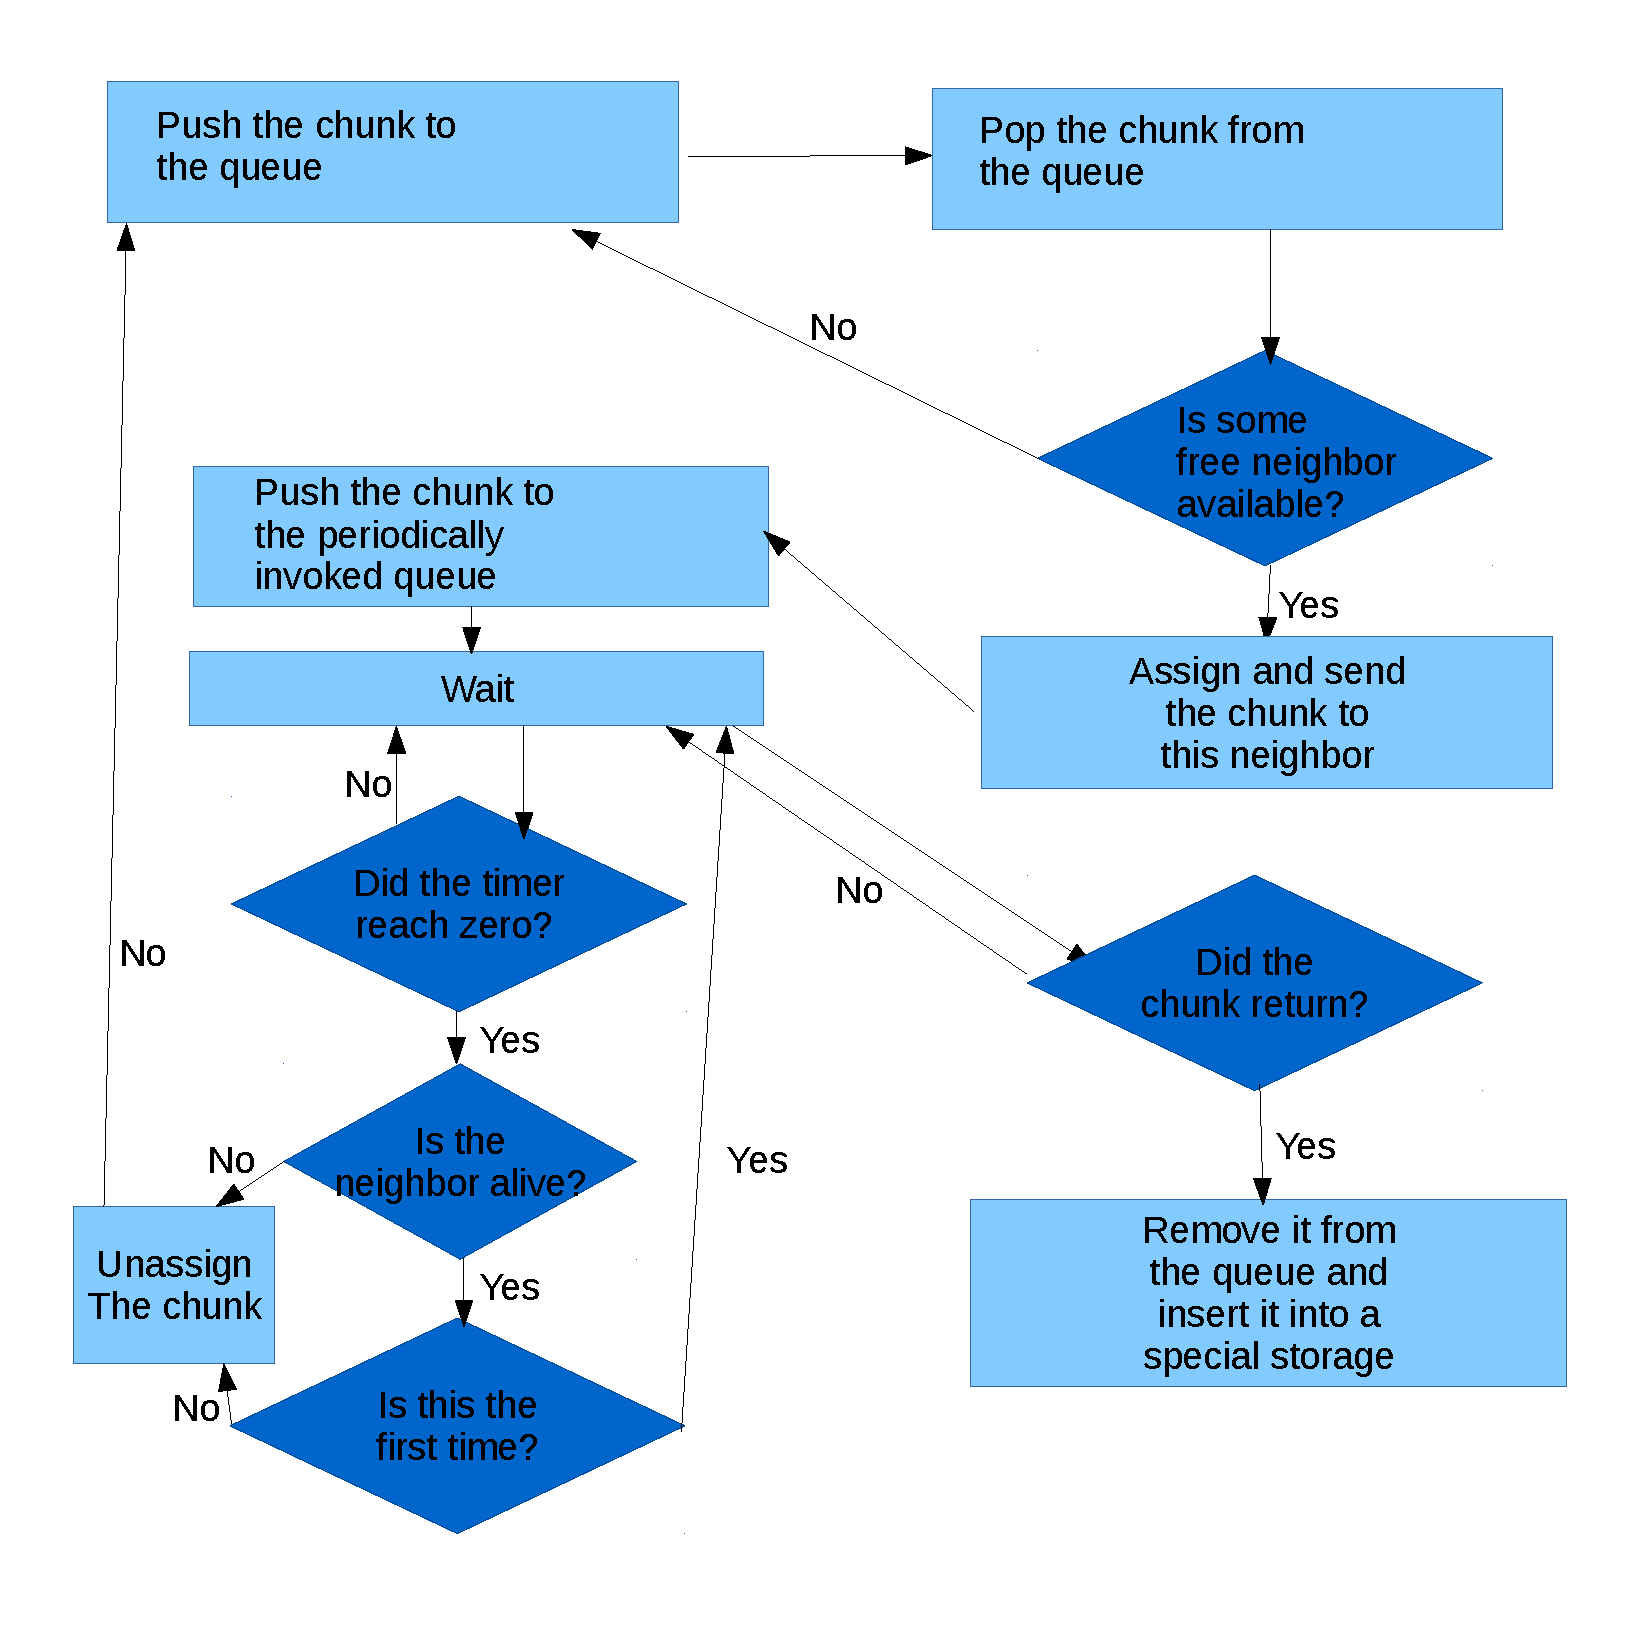
\includegraphics[scale=0.40]{./img/workflow_chunks.pdf}
\caption{Processing a chunk - initiator part}
\end{center}
\end{figure}

\subsection*{Storing files}

Tightly coupled with this process is the problem of storing the files.
Four files have to be created during the processing of every chunk. The
first one is created when the original file is split. This file can't be
removed until the processed chunk returns, because it has to be
available in case that the conversion fails for some reason. Another two
files are created at the processing node, one for the input and one to
store the output. The last file is created at the initiating node again
to hold the processed chunk. This means, that the initiator has to have
free disk space at least twice larger than the resulting file.

\subsection*{Picking neighbors}

Last but not least we have to choose policy to whom the chunks are
distributed. We want to achieve as big speedup as possible, while
preserving rather small list of neighbors. When the chunk is popped out
from the queue, the initiator looks for suitable neighbor. That is the
neighbor which has free status in the corresponding structure. If no
such neighbor is found, the chunk is re-queued and another try is
postponed. Also the gathering process described in the previous section
begins. If some neighbor is available, the chunk is assigned to it and
the transfer may begin. The initiator keeps track how many chunks were
sent to the particular neighbor and it does not send more than specified
count to one neighbor because it could potentially cause delay. The flag
indicating whether the neighbor is free helps to control the flow. Each
time chunk is assigned to the neighbor, the flag is set to false value
to prevent sending more chunks in parallel. It's set to true again after
the successful completion of the transfer. When the neighbor is too
busy, it can express it in the communication, so the flag is set to
false to prevent overloading of the neighbor. The flag is also refreshed
during every periodic check.

\subsection{Security issues}\label{security-issues}

The present implementation is possibly vulnerable to some security
threat. This is caused partly by the pure peer to peer nature, because
it is difficult to control the traffic and authorize all nodes in
dynamic environments like this. It also was not our aim to solve this
issue. The framework is supposed to be used mostly in LANs (Local Area
Network) where all the peers are trustworthy. Otherwise it could be
compromised easily. For example when the encoded chunk arrives, it is
not checked whether it has been sent to this node or not. So a malicious
chunk could be infiltrated causing bad output or even failure of the
joining process.

\subsection{Networking handling}\label{networking-handling}

The network communication is the most important part of the framework.
Standard C library functions and structures were used which are
conforming to
POSIX.1-2001\footnote{https://en.wikipedia.org/wiki/POSIX\#POSIX.1-2001}
standard. Although the program is intended to be used on the
UNIX\footnote{https://en.wikipedia.org/wiki/Unix} or UNIX-like operating
systems, it should be portable to the Microsoft Windows systems as well
thanks to the use of this standard. To preserve simplicity, all the
network communication makes use of the TCP (Transmission Control
Protocol)
\footnote{https://en.wikipedia.org/wiki/Transmission\_Control\_Protocol}.
The system primarily uses the IPv6
\footnote{https://en.wikipedia.org/wiki/Internet\_Protocol} addresses,
but it can be run in the mode which uses addresses of the IPv4 family
only. Additional and more detailed information can be found in
\hyperref[implementation]{chapter 2}.

\subsection{User interface}\label{user-interface}

To provide interaction with the user, the
curses\footnote{https://en.wikipedia.org/wiki/Curses\_(programming\_library)}
library is used. This library makes it possible to control the terminal
screen. That means, the application does not require any special GUI
(Graphical User Interface) libraries and is able to run interactively
even on machines without the X server. The control is rather simple,
offering possibilities to load the file, start or abort the process,
show information about neighbors and so on. The interaction require only
a keyboard, no mouse is needed at all. Concrete information together
with some examples can be found in
\hyperref[installation-and-use]{appendix A}. Detailed information about
the implementation, namely the synchronization problems are discussed in
\hyperref[implementation]{chapter 2}.
